\documentclass[12pt,a4paper]{report}
\usepackage{graphicx}			% Use this package to include images
\usepackage{amsmath}			% A library of many standard math expressions
\usepackage[margin=1in]{geometry}% Sets 1in margins. 
\usepackage{fancyhdr}			% Creates headers and footers
\usepackage{enumerate}          %These two package give custom labels to a list
\usepackage[shortlabels]{enumitem}
\usepackage[utf8]{inputenc}
\usepackage[T1]{fontenc}
\usepackage{amsfonts}
\usepackage{amsmath}
\usepackage{graphicx}
\usepackage{float}
\usepackage{hyperref}
\usepackage{tabularx}
\usepackage[sorting=none]{biblatex}
\usepackage{multicol}
\usepackage{multirow}
\usepackage{xcolor}
\usepackage{pgfplots}
\usepackage{colortbl}
\usepackage{subcaption}
\usepackage[label=corner]{karnaugh-map}
\addbibresource{ref.bib}
\setlength{\columnsep}{20pt}
\setlength{\voffset}{0.7cm}
\setlength{\headsep}{20pt}
\setlength{\headheight}{20pt}
% \usepackage[top=3cm,bottom=2.5cm,left=2.5cm,right=2.5cm,marginparwidth=1.5cm]{geometry}
% Creates the header and footer. You can adjust the look and feel of these here.
\pagestyle{fancy}
\fancyhead[l]{Raymond Timothy Tumiwa}
\fancyhead[c]{ECE4050 Project 1}
\fancyhead[r]{\today}
\fancyfoot[c]{\thepage}
\renewcommand{\headrulewidth}{0.2pt} %Creates a horizontal line underneath the header
\setlength{\headheight}{1pt} %Sets enough space for the header

\begin{document} %The writing for your homework should all come after this. 


\begin{titlepage}
 \centering
    
\includegraphics[scale = 0.75,width=6cm]{CUHK}\\[1.0 cm] % University Logo}
    \textsc{\large The Chinese University of Hong Kong, Shenzhen}\\[2.0 cm] 
    \textsc{\Large ECE4050}\\[0.5 cm] % Course Code
    \textsc{\large Principles and Practices of Network Communications}\\[0.5 cm] % Course Name
    \rule{\linewidth}{0.2 mm} \\[0.5 cm]
    {\Large \textbf{Project 1 \\ Network Simulator \textit{\textbf{ns.py}} }}\\[0.5cm]
    \rule{\linewidth}{0.2 mm} \\[1.5 cm]
    
    \begin{minipage}{0.4\textwidth}
        \begin{flushleft} \large
            \emph{Author:}\\
            {Raymond Timothy Tumiwa}
            \end{flushleft}
    \end{minipage}~
    \begin{minipage}{0.4\textwidth}
            \begin{flushright} \large
            \emph{Student Number:} \\
            121010002  % Modify your student number
        \end{flushright}
    \end{minipage}\\[0.5cm]
    
    {\large{3 March 2024}}\\[2 cm]
 
    \vfill
\end{titlepage}
\subsection*{Introduction}
\noindent The project explores \textit{\textbf{ns.py}}, a network simulator that simulates how the congestion control algorithm works in the network environment. This project's transmission control protocol (TCP) analyzes the Reno and Cubic congestion control algorithms. The project report will analyze their (reno and cubic) performance in handling network traffic with different congestion control algorithms and how they operate. There are two different results together with two different data to be considered. The result is from two different methods where the first method is when S1 and S2 use both Reno as the congestion control, and the second one is when S1 use Reno while S2 use Cubic. The data that will be analyzed are the average throughput within the two receivers (flow sending rate) and the congestion window size. 
\subsection*{S1 Reno with S2 Reno}
The first result is shown in the two figures below, figure \ref{fig: result_rr_1} and \ref{fig: result_rr_2}.  Sink 1 and Sink 2 have an almost identical average rate of data receipt, with the oscillating data around 9000 to 11000 bytes per second, calculated over the last 10 packets. This metric measures the network's performance, indicating how quickly the sink receives data at that moment. It reflects the data rate over a short, recent interval. Both throughputs start with slower rates, around 4000, rising to 6000 and then to 11000 because of the window size increase. There is a slight difference where S2 output reaches a point around 14000 that might be caused by too much data sent or just a simple error, but the data is still consistent as it eventually goes back to the normal maximum rate around 9000 to 11000.\\
\begin{figure}[!ht]
\begin{subfigure}{0.5\textwidth}
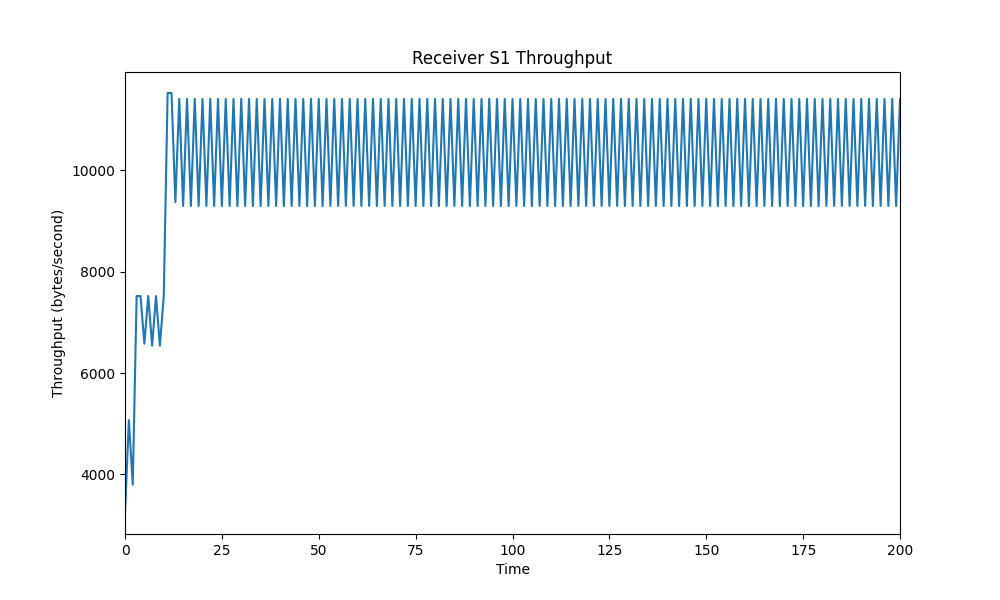
\includegraphics[width=1\linewidth, height=5cm]{Pictures/S1_Reno_Throughput.png} 
\caption{Reno S1 Average Throughput}
\end{subfigure}
\begin{subfigure}{0.5\textwidth}
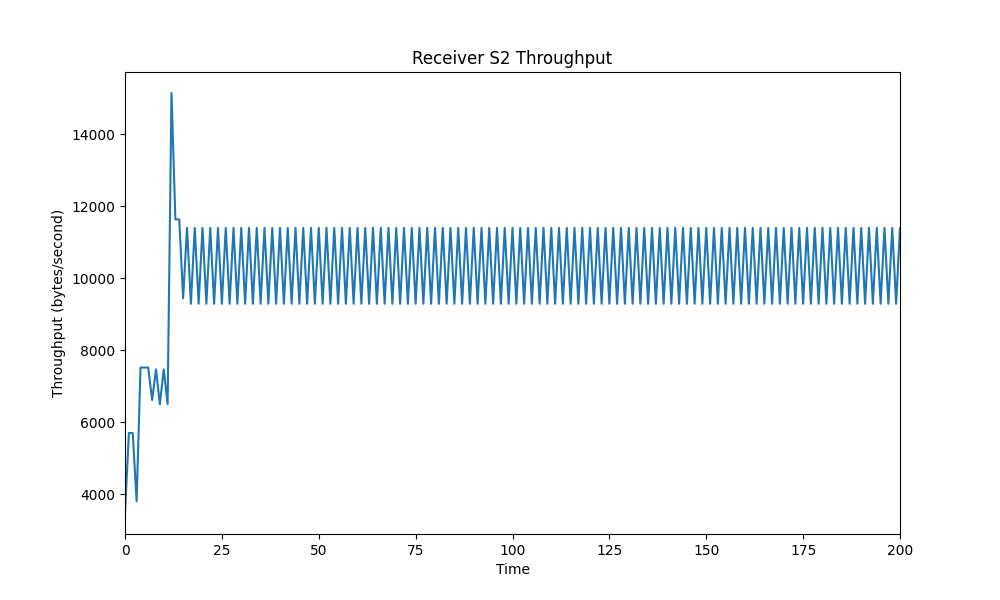
\includegraphics[width=1\linewidth, height=5cm]{Pictures/S2_Reno_Throughput.png}
\caption{Reno S2 Average Throughput}
\end{subfigure}
\caption{Reno - Reno Average Throughput Rate}
\label{fig: result_rr_1}
\end{figure}
\break
\noindent The two figures above show that the throughput oscillates between high and low rates. It suggests that the throughput will go up whenever there is no congestion and down whenever congestion exists. This also suggests the window size increases and decreases depending on the throughput rate. However, compared to the figure \ref{fig: result_rr_2}, the congestion window keeps increasing while the throughput is sawed tooth shape. One possible cause of this inconsistency is that the switch that acts as the forwarding message has too high a port rate, which causes no congestion of the forwarding. Hence, the congestion window size can keep increasing without ever experiencing congestion.\\
Figure \ref{fig: result_rr_2} shows that the congestion window size increases for both TCP packet generators, stabilising at a high value. This suggests that the TCP algorithm has reached a state where it believes the network can handle a large amount of data without causing congestion. The Reno system initially increases the window as fast as it can but starts to increase linearly when congestion happens.\\
\begin{figure}[!ht]
\begin{subfigure}{0.5\textwidth}
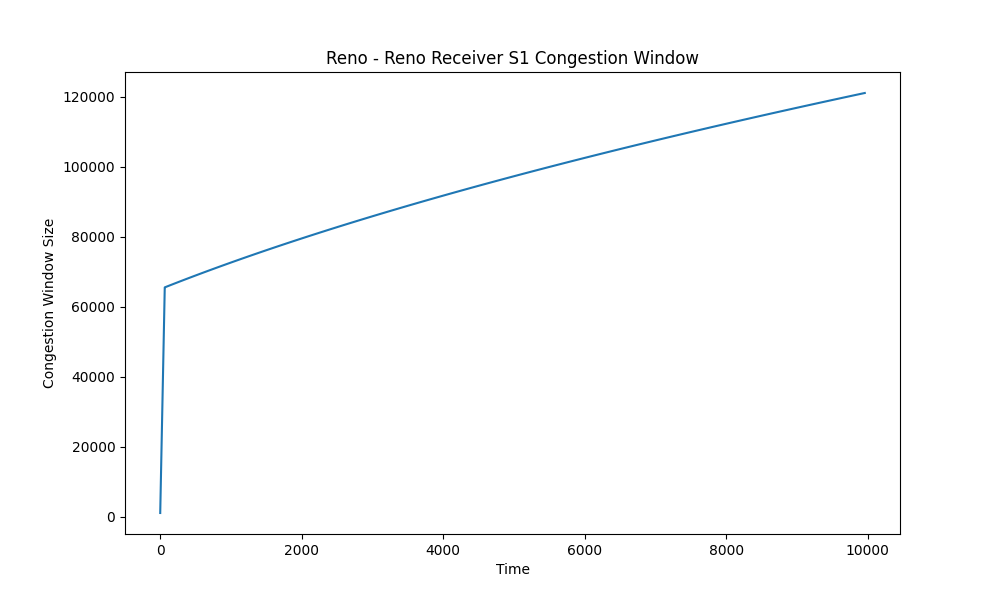
\includegraphics[width=1\linewidth, height=6cm]{Pictures/S1_Reno_Window.png} 
\caption{Reno S1 Window Size}
\end{subfigure}
\begin{subfigure}{0.5\textwidth}
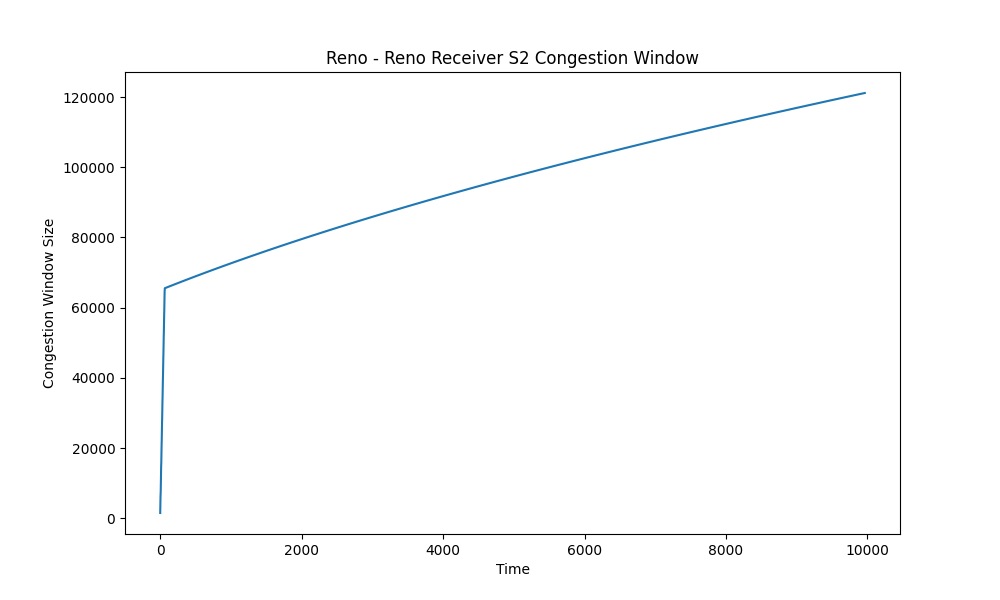
\includegraphics[width=1\linewidth, height=6cm]{Pictures/S2_Reno_Window.png}
\caption{Reno S2 Window Size}
\end{subfigure}
\caption{Reno - Reno Congestion Window Size}
\label{fig: result_rr_2}
\end{figure}
\subsection*{S1 Reno with S2 Cubic}
The second result is shown in the two figures below, figure \ref{fig: result_rc_1} and \ref{fig: result_rc_2}.  Sink 1 and Sink 2 have an identical average rate of data receipt that oscillates between 9000 and 11000 bytes per second, calculated over the last 10 packets. As explained in part one, S1 Reno with S2 Reno, the throughput starts slower, increasing periodically and maintaining a certain saw-tooth point of 9000 to 11000. \\
\begin{figure}[!ht]
\begin{subfigure}{0.5\textwidth}
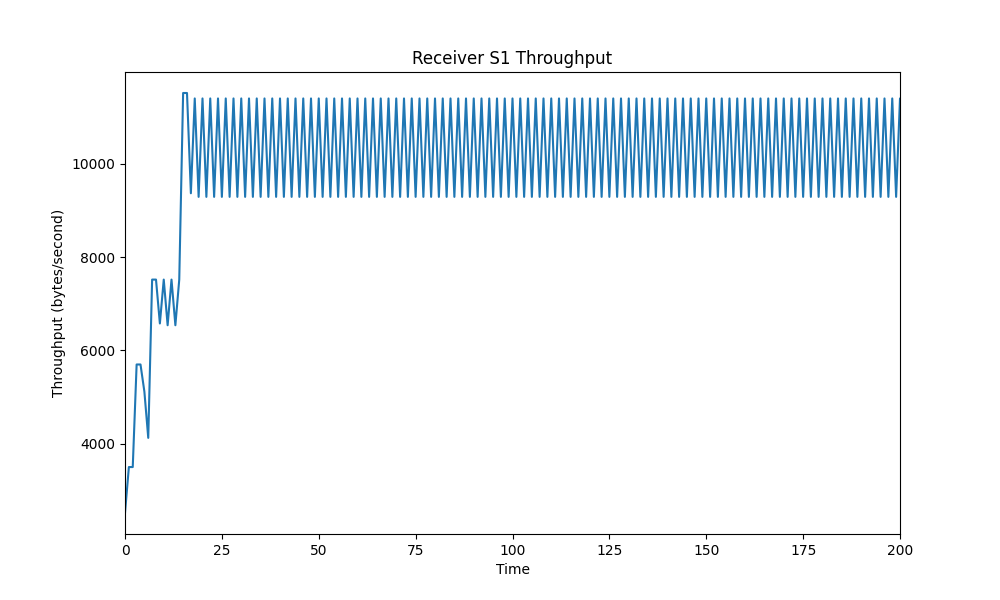
\includegraphics[width=1\linewidth, height=6cm]{Pictures/S1_Cubic_Throughput.png} 
\caption{Reno S1 Average Throughput}
\end{subfigure}
\begin{subfigure}{0.5\textwidth}
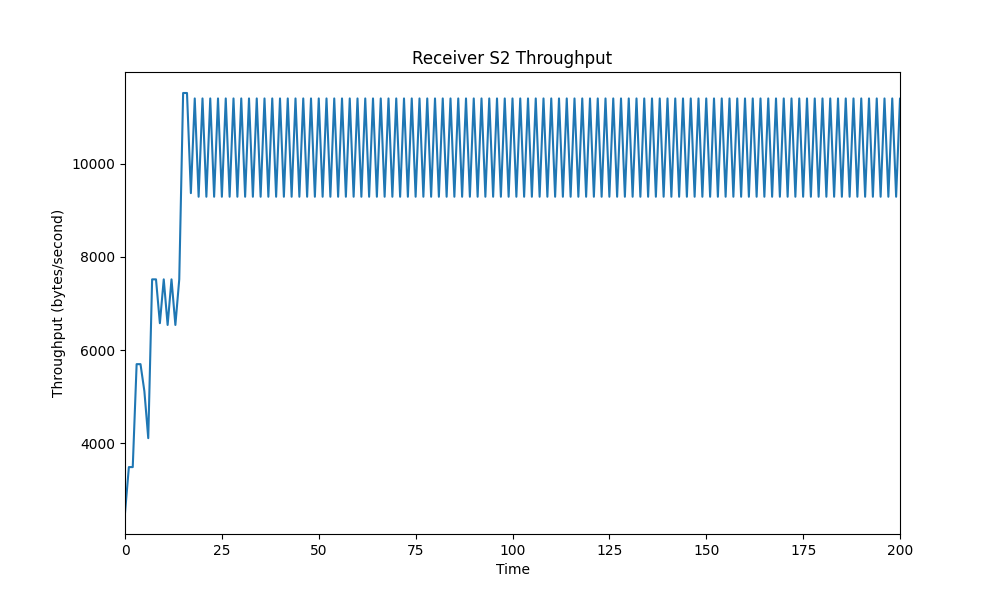
\includegraphics[width=1\linewidth, height=6cm]{Pictures/S2_Cubic_Throughput.png}
\caption{Cubic S2 Average Throughput}
\end{subfigure}
\caption{Reno - Cubic Average Throughput Rate}
\label{fig: result_rc_1}
\end{figure}
\break
\noindent As stated before, the two figures above show that the throughput oscillates between high and low rates. It suggests that the throughput will go up whenever there is no congestion and down whenever congestion exists. This also suggests the window size increases and decreases depending on the throughput rate. However, compared to the figure \ref{fig: result_rc_2}, the congestion window keeps increasing while the throughput is sawed tooth shape. As explained before, one possible cause of this inconsistency is that the switch acting as the forwarding message has too high a port rate, which causes no congestion of the forwarding. Hence, the congestion window size can keep increasing without ever experiencing congestion.\\
Figure \ref{fig: result_rc_2} shows that the congestion window size increases for both TCP packet generators, stabilising at a high value just as how the first data works. This suggests that the TCP algorithm has reached a state where it believes the network can handle a large amount of data without causing congestion. However, there is a slight difference in the window size between S1 (Reno) and S2 (Cubic). As explained before, the Reno system increases linearly during congestion. On the other hand, the cubic function allows the window to grow rapidly in environments with large amounts of available bandwidth. Still, it ensures that it does not increase as aggressively as the available bandwidth gets filled to avoid causing congestion. Hence, as seen in the window size graph, the Reno window is higher during the first period. Still, eventually, the Cubic window size grows exponentially faster and much larger than Reno. \break \hfill 
\begin{figure}[!ht]
\begin{subfigure}{0.5\textwidth}
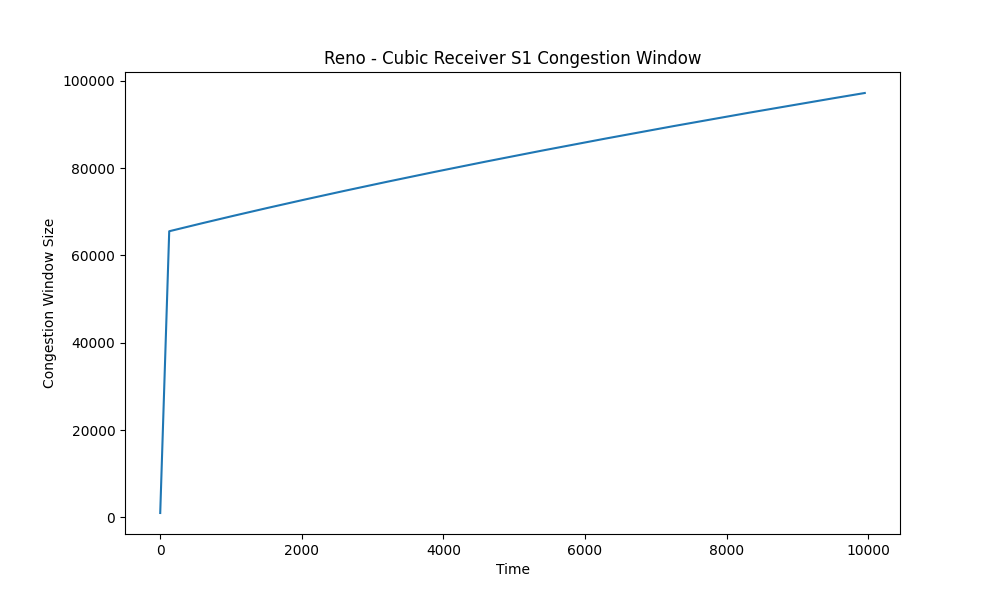
\includegraphics[width=1\linewidth, height=6cm]{Pictures/S1_Cubic_Window.png} 
\caption{Reno S1 Window Size}
\end{subfigure}
\begin{subfigure}{0.5\textwidth}
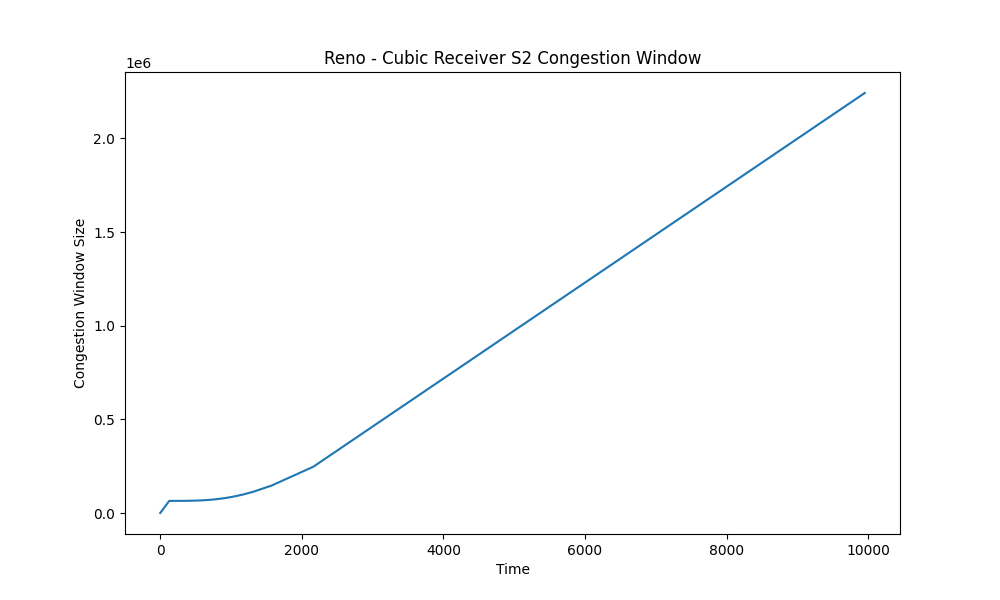
\includegraphics[width=1\linewidth, height=6cm]{Pictures/S2_Cubic_Window.png}
\caption{Cubic S2 Window Size}
\end{subfigure}
\caption{Reno - Cubic Congestion Window Size}
\label{fig: result_rc_2}
\end{figure}
\subsection*{Conclusion}
In conclusion, this project analysed the Reno and Cubic TCP congestion control algorithms through \textit{\textbf{ns.py}} simulations. It has been observed that while both algorithms aim to optimize throughput while minimizing congestion, their approaches and resulting performances differ significantly. Reno's conservative linear increase to avoid packet loss during congestion might not be optimal for high-bandwidth networks. With its more aggressive window growth function, Cubic is better suited for modern, high-bandwidth networks, achieving higher throughput without inducing congestion. However, it also becomes evident that the inherent increase in window size does not always correlate with improved throughput due to factors like receiver constraints or protocol overhead. Future improvements to this project could involve incorporating more diverse network conditions, including varying latencies and packet loss scenarios, to challenge further and analyse each algorithm's robustness and efficiency. One way to produce packet loss scenarios is by incorporating a lower switch port rate.

\end{document}
